\tableofcontents

\newpage

\section{Задание}
По выданному преподавателем варианту восстановить текст заданного варианта программы и подпрограммы (программного комплекса), определить предназначение и составить его описание, определить область представления и область допустимых значений исходных данных и результата, выполнить трассировку программного комплекса.
\begin{figure}[H]
\centering
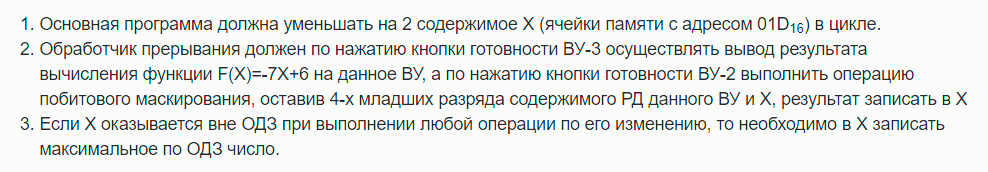
\includegraphics[scale=0.6]{task}
\label{pic:task}
\end{figure}

\section{Текст программного комплекса}

\subsection{Текст программы}
\begin{center}
\begin{tabular}{|c|c|c|l|}
\hline
\textbf{Адрес ячейки} & \textbf{Содержимое ячейки} & \textbf{Мнемоника} & \textbf{Комментарии}\\
\hline
149 & 0200 & CLA & Очищаем аккумулятор и\\
14A & EE19 & ST IP$+$25 & загружаем ноль в ячейку 164\\
14B & AE17 & LD IP$+$23 & Загружаем первый аргумент\\
14C & 0C00 & PUSH & подпрограммы (ячейка 163) в стек\\
14D & D690 & CALL 0x690 & Запускаем подпрограмму с началом в 0x690\\
14E & 0800 & POP & Выгружаем выходные данные подпрограммы\\
14F & 0700 & INC & и увеличиваем их на единицу\\
150 & 6E13 & SUB IP$+$19 & Вычитаем нулевое значение ячейки 164\\
151 & EE12 & ST IP$+$18 & Сохраняем результат в ячейку 164\\
152 & AE0E & LD IP$+$14 & Загружаем второй аргумент\\
153 & 0C00 & PUSH & подпрограммы (ячейка 161) в стек\\
154 & D690 & CALL 0x690 & Запускаем подпрограмму с началом в 0x690\\
155 & 0800 & POP & Выгружаем выходные данные подпрограммы\\
156 & 6E0D & SUB IP$+$13 & Вычитаем текущее значение ячейки 164\\
157 & EE0C & ST IP$+$12 & Сохраняем результат в ту же ячейку\\
158 & AE09 & LD IP$+$9 & Загружаем уменьшенный на\\
159 & 0740 & DEC & единицу  третий аргумент\\
15A & 0C00 & PUSH & подпрограммы (ячейка 162) в стек\\
15B & D690 & CALL 0x690 & Запускаем подпрограмму с началом в 0x690\\
15C & 0800 & POP & Выгружаем выходные данные подпрограммы\\
15D & 0700 & INC & и увеличиваем их на единицу\\
15E & 6E05 & SUB IP$+$5 & Вычитаем текущее значение ячейки 164\\
15F & EE04 & ST IP$+$4 & Сохраняем результат в ту же ячейку\\
160 & 0100 & HLT & Завершаем программу\\
\hline
161 & A51A & Z & Второй аргумент подпрограммы\\
162 & 1DEA & Y & Третий аргумент подпрограммы\\
163 & 0BA3 & X & Первый аргумент подпрограммы\\
164 & 0BF2 & R & Результат работы программы\\
\hline
\end{tabular}
\end{center}

\newpage

\subsection{Текст подпрограммы}
\begin{center}
\begin{tabular}{|c|c|c|l|}
\hline
\textbf{Адрес ячейки} & \textbf{Содержимое ячейки} & \textbf{Мнемоника} & \textbf{Комментарии}\\
\hline
690 & AC01 & LD \&1 & Загружаем аргумент подпрограммы\\
691 & F207 & BMI IP$+$7 & Если число неположительное, то\\
692 & F006 & BEQ IP$+$6 & переходим к ячейке 699\\
693 & 7E08 & CMP IP$+$8 & Если аргумент больше или равен U, то\\
694 & F904 & BGE IP$+$4 & переходим к ячейке 699\\
695 & 0500 & ASL & Если ни одно условие не\\
696 & 4C01 & ADD \&1 & выполнилось, то умножаем аргумент на 4\\
697 & 6E05 & SUB IP$+$5 & Вычитаем локальную переменную W\\
698 & CE01 & BR IP$+$1 & Переходим к ячейке 699\\
699 & AE02 & LD IP$+$2 & Загружаем локальную переменную U\\
69A & EC01 & ST \&1 & Сохраняем результат в стек\\
69B & 0A00 & RET & Возврат из подпрограммы\\
\hline
69C & 0BF0 & U & Локальная переменная, U $=const=3056$\\
69D & 0047 & W & Локальная переменная, W $=const=71$\\
\hline
\end{tabular}
\end{center}

\section{Описание программного комплекса}
\subsection{Назначение и реализуемые функции}
\subsubsection{Реализуемая программой функция}
$$R=F(X)+F(Y-1)-F(Z)+2$$

\subsubsection{Реализуемая подпрограммой функция}
\begin{center}
$F(X) = \begin{cases}
3056 & \text{при } X \leqslant 0,\\
4X-71 & \text{при } 0<X<3056,\\
3056 & \text{при } X \geqslant 3056.
\end{cases}$
\end{center}

\subsubsection{Реализуемый подпрограммой график функции}
\begin{figure}[H]
\centering
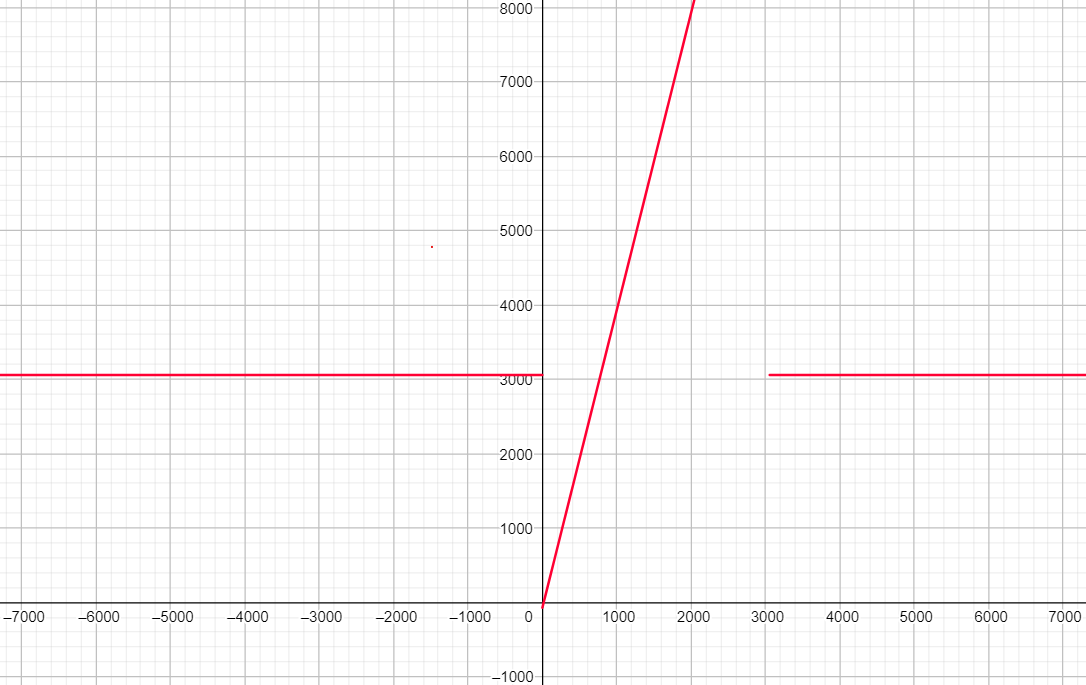
\includegraphics[scale=0.7]{graphic}
\label{pic:graphic}
\end{figure}

\subsection{Область представления и область допустимых значений данных}
\subsubsection{Область представления данных}
\noindent Ячейки Z, Y, X, R: 16-разрядные знаковые целые числа в диапазоне $-2^{15}\ldots2^{15}-1$

\subsubsection{Область допустимых значений данных}
\noindent $min(F(X))=-67$\\
$max(F(X))=12149$\\
$\Rightarrow Z, Y, X, R \in [-2^{15}; 2^{15}-1]$

\subsection{Расположение в памяти ЭВМ}
\noindentПрограмма: 149\ldots160\\
Первый аргумент подпрограммы (X): 163\\
Второй аргумент подпрограммы (Z): 161\\
Третий аргумент подпрограммы (Y): 162\\
Результат работы программы: 164\\

\noindentПодпрограмма: 690\ldots69B\\
Локальная переменная U $=3056$: 69C\\
Локальная переменная W $=71$: 69D

\subsection{Адреса первой и последней выполняемой команд}
\noindent Адрес первой команды программы: 149\\
Адрес последней команды программы: 160

\section{Таблица трассировки}
\begin{center}
\begin{tabular}{|c|c|c|c|c|c|c|c|c|c|c|c|}
\hline
\multicolumn{2}{|c}{\makecell{\textbf{Выполняемая}\\\textbf{команда}}}
  &\multicolumn{8}{|c|}{\textbf{Содердимое регистров после выполнения команды}}
  &\multicolumn{2}{c|}{\makecell{\textbf{Ячейка, содержимое}\\\textbf{которой изменилось}}}\\
\hline
Адрес & Код & IP & CR & AR & DR & SP & BR & AC & NZVC & Адрес & Новый код\\
\hline
149 & 0200 & 149 & 0000 & 000 & 0000 & 000 & 0000 & 0000 & 0100 & --- & ---\\
\hline
149 & 0200 & 14A & 0200 & 149 & 0200 & 000 & 0149 & 0000 & 0100 & --- & ---\\
\hline
14A & EE19 & 14B & EE19 & 164 & 0000 & 000 & 0019 & 0000 & 0100 & 164 & 0000\\
\hline
14B & AE17 & 14C & AE17 & 163 & 0BA3 & 000 & 0017 & 0BA3 & 0000 & --- & ---\\
\hline
14C & 0C00 & 14D & 0C00 & 7FF & 0BA3 & 7FF & 014C & 0BA3 & 0000 & 7FF & 0BA3\\
\hline
14D & D690 & 690 & D690 & 7FE & 014E & 7FE & D690 & 0BA3 & 0000 & 7FE & 014E\\
\hline
690 & AC01 & 691 & AC01 & 7FF & 0BA3 & 7FE & 0001 & 0BA3 & 0000 & --- & ---\\
\hline
691 & F207 & 692 & F207 & 691 & F207 & 7FE & 0691 & 0BA3 & 0000 & --- & ---\\
\hline
692 & F006 & 693 & F006 & 692 & F006 & 7FE & 0692 & 0BA3 & 0000 & --- & ---\\
\hline
693 & 7E08 & 694 & 7E08 & 69C & 0BF0 & 7FE & 0008 & 0BA3 & 1000 & --- & ---\\
\hline
694 & F904 & 695 & F904 & 694 & F904 & 7FE & 0694 & 0BA3 & 1000 & --- & ---\\
\hline
695 & 0500 & 696 & 0500 & 695 & 0BA3 & 7FE & 0695 & 1746 & 0000 & --- & ---\\
\hline
696 & 4C01 & 697 & 4C01 & 7FF & 0BA3 & 7FE & 0001 & 22E9 & 0000 & --- & ---\\
\hline
697 & 6E05 & 698 & 6E05 & 69D & 0047 & 7FE & 0005 & 22A2 & 0001 & --- & ---\\
\hline
698 & CE01 & 69A & CE01 & 698 & 069A & 7FE & 0001 & 22A2 & 0001 & --- & ---\\
\hline
69A & EC01 & 69B & EC01 & 7FF & 22A2 & 7FE & 0001 & 22A2 & 0001 & 7FF & 22A2\\
\hline
69B & 0A00 & 14E & 0A00 & 7FE & 014E & 7FF & 069B & 22A2 & 0001 & --- & ---\\
\hline
14E & 0800 & 14F & 0800 & 7FF & 22A2 & 000 & 014E & 22A2 & 0001 & --- & ---\\
\hline
14F & 0700 & 150 & 0700 & 14F & 0700 & 000 & 014F & 22A3 & 0000 & --- & ---\\
\hline
150 & 6E13 & 151 & 6E13 & 164 & 0000 & 000 & 0013 & 22A3 & 0001 & --- & ---\\
\hline
151 & EE12 & 152 & EE12 & 164 & 22A3 & 000 & 0012 & 22A3 & 0001 & 164 & 22A3\\
\hline
152 & AE0E & 153 & AE0E & 161 & A51A & 000 & 000E & A51A & 1001 & --- & ---\\
\hline
153 & 0C00 & 154 & 0C00 & 7FF & A51A & 7FF & 0153 & A51A & 1001 & 7FF & A51A\\
\hline
154 & D690 & 690 & D690 & 7FE & 0155 & 7FE & D690 & A51A & 1001 & 7FE & 0155\\
\hline
690 & AC01 & 691 & AC01 & 7FF & A51A & 7FE & 0001 & A51A & 1001 & --- & ---\\
\hline
691 & F207 & 699 & F207 & 691 & F207 & 7FE & 0007 & A51A & 1001 & --- & ---\\
\hline
699 & AE02 & 69A & AE02 & 69C & 0BF0 & 7FE & 0002 & 0BF0 & 0001 & --- & ---\\
\hline
69A & EC01 & 69B & EC01 & 7FF & 0BF0 & 7FE & 0001 & 0BF0 & 0001 & 7FF & 0BF0\\
\hline
69B & 0A00 & 155 & 0A00 & 7FE & 0155 & 7FF & 069B & 0BF0 & 0001 & --- & ---\\
\hline
155 & 0800 & 156 & 0800 & 7FF & 0BF0 & 000 & 0155 & 0BF0 & 0001 & --- & ---\\
\hline
156 & 6E0D & 157 & 6E0D & 164 & 22A3 & 000 & 000D & E94D & 1000 & --- & ---\\
\hline
157 & EE0C & 158 & EE0C & 164 & E94D & 000 & 000C & E94D & 1000 & 164 & E94D\\
\hline
158 & AE09 & 159 & AE09 & 162 & 1DEA & 000 & 0009 & 1DEA & 0000 & --- & ---\\
\hline
159 & 0740 & 15A & 0740 & 159 & 0740 & 000 & 0159 & 1DE9 & 0001 & --- & ---\\
\hline
15A & 0C00 & 15B & 0C00 & 7FF & 1DE9 & 7FF & 015A & 1DE9 & 0001 & 7FF & 1DE9\\
\hline
15B & D690 & 690 & D690 & 7FE & 015C & 7FE & D690 & 1DE9 & 0001 & 7FE & 015C\\
\hline
690 & AC01 & 691 & AC01 & 7FF & 1DE9 & 7FE & 0001 & 1DE9 & 0001 & --- & ---\\
\hline
691 & F207 & 692 & F207 & 691 & F207 & 7FE & 0691 & 1DE9 & 0001 & --- & ---\\
\hline
692 & F006 & 693 & F006 & 692 & F006 & 7FE & 0692 & 1DE9 & 0001 & --- & ---\\
\hline
693 & 7E08 & 694 & 7E08 & 69C & 0BF0 & 7FE & 0008 & 1DE9 & 0001 & --- & ---\\
\hline
694 & F904 & 699 & F904 & 694 & F904 & 7FE & 0004 & 1DE9 & 0001 & --- & ---\\
\hline
699 & AE02 & 69A & AE02 & 69C & 0BF0 & 7FE & 0002 & 0BF0 & 0001 & --- & ---\\
\hline
69A & EC01 & 69B & EC01 & 7FF & 0BF0 & 7FE & 0001 & 0BF0 & 0001 & 7FF & 0BF0\\
\hline
69B & 0A00 & 15C & 0A00 & 7FE & 015C & 7FF & 069B & 0BF0 & 0001 & --- & ---\\
\hline
15C & 0800 & 15D & 0800 & 7FF & 0BF0 & 000 & 015C & 0BF0 & 0001 & --- & ---\\
\hline
15D & 0700 & 15E & 0700 & 15D & 0700 & 000 & 015D & 0BF1 & 0000 & --- & ---\\
\hline
15E & 6E05 & 15F & 6E05 & 164 & E94D & 000 & 0005 & 22A4 & 0000 & --- & ---\\
\hline
15F & EE04 & 160 & EE04 & 164 & 22A4 & 000 & 0004 & 22A4 & 0000 & 164 & 22A4\\
\hline
160 & 0100 & 161 & 0100 & 160 & 0100 & 000 & 0160 & 22A4 & 0000 & --- & ---\\
\hline
\end{tabular}
\end{center}

\section{Вывод}
В ходе данной лабораторной работы я познакомился с использованием подпрограмм в БЭВМ, работой стека и новыми для меня командами - CALL, RET, PUSH и POP. Эти знания пригодятся мне для дальнейшей работы с БЭВМ и понимания работы современных ЭВМ.
